\documentclass[twocolumn]{article}
\usepackage[utf8]{inputenc}
\usepackage{amsmath,amssymb}
\usepackage{booktabs}
\usepackage{tikz}
\usepackage{pgfplots}
\pgfplotsset{compat=1.18}
\usetikzlibrary{calc,positioning,patterns}

% Professional A* Color Palette
\definecolor{oursblue}{RGB}{46,111,183}
\definecolor{vllmred}{RGB}{209,73,91}
\definecolor{basegray}{RGB}{154,164,174}
\definecolor{boundorange}{RGB}{224,164,58}
\definecolor{traingreen}{RGB}{89,161,79}

\title{\textbf{Slakshna: P2P Federated Inference Figures Preview}}
\author{Research Team}
\date{}

\begin{document}
\maketitle

\section{Selection Method Comparison}
\begin{figure}[h]
\centering
% TikZ Figure: Accuracy by Selection Method (AG News)
% Usage: \input{tikzfigs/fig_accuracy_by_selection_method.tex}
% Self-contained color definitions
\providecolor{oursblue}{RGB}{46,111,183}
\providecolor{boundorange}{RGB}{224,164,58}
\providecolor{vllmred}{RGB}{209,73,91}
\providecolor{basegray}{RGB}{154,164,174}
\providecolor{traingreen}{RGB}{89,161,79}
\resizebox{\linewidth}{!}{%
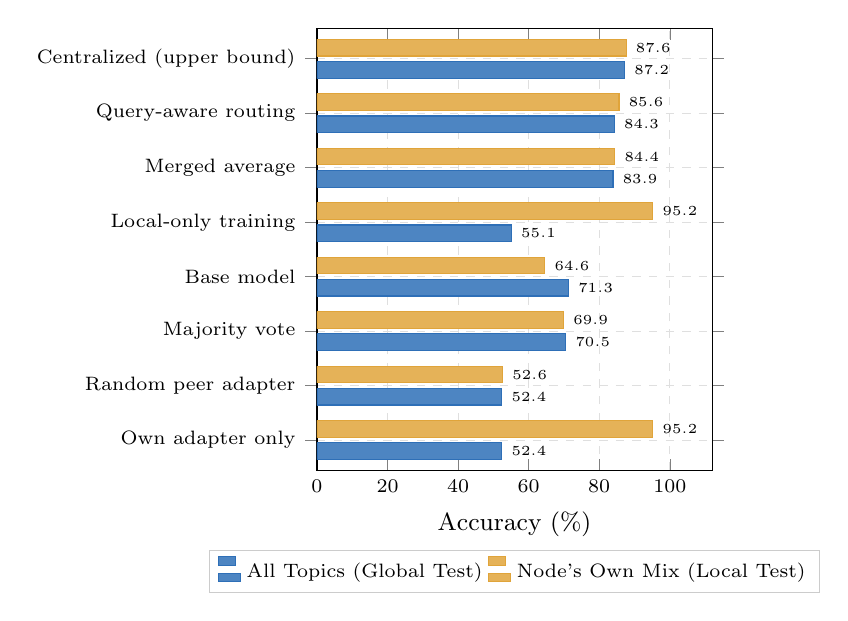
\begin{tikzpicture}
\begin{axis}[
    xbar,
    width=6.6cm,
    height=7.2cm,
    xmin=0, xmax=112,
    xtick={0, 20, 40, 60, 80, 100},
    xlabel={Accuracy (\%)},
    symbolic y coords={
        {Own adapter only},
        {Random peer adapter},
        {Majority vote},
        {Base model},
        {Local-only training},
        {Merged average},
        {Query-aware routing},
        {Centralized (upper bound)}
    },
    ytick=data,
    yticklabel style={font=\scriptsize, align=right},
    xticklabel style={font=\scriptsize},
    xlabel style={font=\small},
    nodes near coords,
    nodes near coords style={font=\tiny, text=black, anchor=west},
    nodes near coords align={horizontal},
    point meta=rawx,
    bar width=6pt,
    enlarge y limits=0.08,
    legend style={font=\scriptsize, at={(0.5,-0.18)}, anchor=north, legend columns=2, draw=gray!40, fill=white},
    grid=major,
    grid style={dashed, gray!25}
]

% All Topics (Global Balanced Test Set)
\addplot[fill=oursblue!85, draw=oursblue] coordinates {
    (52.4,{Own adapter only})
    (52.4,{Random peer adapter})
    (70.5,{Majority vote})
    (71.3,{Base model})
    (55.1,{Local-only training})
    (83.9,{Merged average})
    (84.3,{Query-aware routing})
    (87.2,{Centralized (upper bound)})
};

% Node's Own Mix (Local Skewed Test Set)
\addplot[fill=boundorange!85, draw=boundorange] coordinates {
    (95.2,{Own adapter only})
    (52.6,{Random peer adapter})
    (69.9,{Majority vote})
    (64.6,{Base model})
    (95.2,{Local-only training})
    (84.4,{Merged average})
    (85.6,{Query-aware routing})
    (87.6,{Centralized (upper bound)})
};

\legend{All Topics (Global Test), Node's Own Mix (Local Test)}
\end{axis}
\end{tikzpicture}%
}

\caption{Accuracy across adapter selection strategies on AG News.}
\label{fig:accuracy_by_selection}
\end{figure}

\section{Topic Specialization Matrix}
\begin{figure}[h]
\centering
% TikZ Figure: Topic Specialization Matrix (AG News)
% Usage: \input{tikzfigs/fig_accuracy_per_topic.tex}
% Self-contained color definitions
\providecolor{oursblue}{RGB}{46,111,183}
\providecolor{boundorange}{RGB}{224,164,58}
\providecolor{vllmred}{RGB}{209,73,91}
\providecolor{basegray}{RGB}{154,164,174}
\providecolor{traingreen}{RGB}{89,161,79}
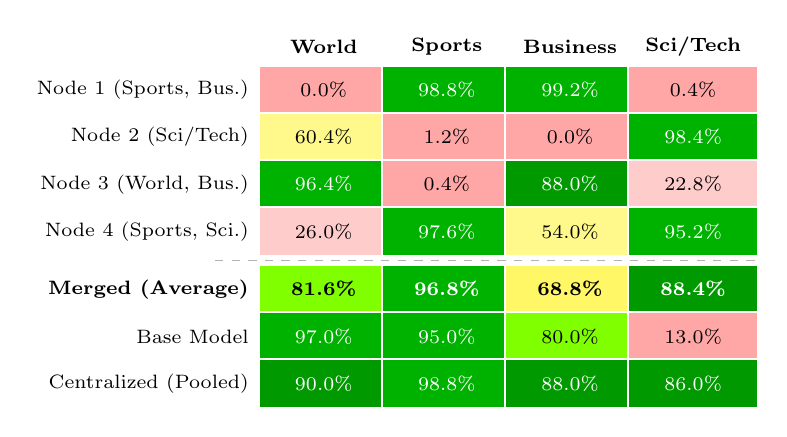
\begin{tikzpicture}[scale=0.92]
\tikzset{
    cell/.style={rectangle, minimum width=1.65cm, minimum height=0.62cm, draw=white, line width=0.8pt, font=\scriptsize, align=center},
    rowlabel/.style={font=\scriptsize, anchor=east, align=right},
    collabel/.style={font=\scriptsize\bfseries, align=center}
}

% Column Headers
\node[collabel] at (1.5, 0.6) {World};
\node[collabel] at (3.2, 0.6) {Sports};
\node[collabel] at (4.9, 0.6) {Business};
\node[collabel] at (6.6, 0.6) {Sci/Tech};

% Row 1: Node 1 (Sports, Business)
\node[rowlabel] at (0.6, 0.0) {Node 1 (Sports, Bus.)};
\node[cell, fill=red!35] at (1.5, 0.0) {0.0\%};
\node[cell, fill=green!70!black, text=white] at (3.2, 0.0) {98.8\%};
\node[cell, fill=green!70!black, text=white] at (4.9, 0.0) {99.2\%};
\node[cell, fill=red!35] at (6.6, 0.0) {0.4\%};

% Row 2: Node 2 (Sci/Tech)
\node[rowlabel] at (0.6, -0.65) {Node 2 (Sci/Tech)};
\node[cell, fill=yellow!45] at (1.5, -0.65) {60.4\%};
\node[cell, fill=red!35] at (3.2, -0.65) {1.2\%};
\node[cell, fill=red!35] at (4.9, -0.65) {0.0\%};
\node[cell, fill=green!70!black, text=white] at (6.6, -0.65) {98.4\%};

% Row 3: Node 3 (World, Business)
\node[rowlabel] at (0.6, -1.30) {Node 3 (World, Bus.)};
\node[cell, fill=green!70!black, text=white] at (1.5, -1.30) {96.4\%};
\node[cell, fill=red!35] at (3.2, -1.30) {0.4\%};
\node[cell, fill=green!60!black, text=white] at (4.9, -1.30) {88.0\%};
\node[cell, fill=red!20] at (6.6, -1.30) {22.8\%};

% Row 4: Node 4 (Sports, Sci/Tech)
\node[rowlabel] at (0.6, -1.95) {Node 4 (Sports, Sci.)};
\node[cell, fill=red!20] at (1.5, -1.95) {26.0\%};
\node[cell, fill=green!70!black, text=white] at (3.2, -1.95) {97.6\%};
\node[cell, fill=yellow!45] at (4.9, -1.95) {54.0\%};
\node[cell, fill=green!70!black, text=white] at (6.6, -1.95) {95.2\%};

% Separator line
\draw[gray!60, dashed, line width=0.5pt] (0.0, -2.35) -- (7.5, -2.35);

% Row 5: All Adapters Merged
\node[rowlabel] at (0.6, -2.75) {\bfseries Merged (Average)};
\node[cell, fill=green!50!yellow] at (1.5, -2.75) {\bfseries 81.6\%};
\node[cell, fill=green!70!black, text=white] at (3.2, -2.75) {\bfseries 96.8\%};
\node[cell, fill=yellow!60] at (4.9, -2.75) {\bfseries 68.8\%};
\node[cell, fill=green!60!black, text=white] at (6.6, -2.75) {\bfseries 88.4\%};

% Row 6: Base Model
\node[rowlabel] at (0.6, -3.40) {Base Model};
\node[cell, fill=green!70!black, text=white] at (1.5, -3.40) {97.0\%};
\node[cell, fill=green!70!black, text=white] at (3.2, -3.40) {95.0\%};
\node[cell, fill=green!50!yellow] at (4.9, -3.40) {80.0\%};
\node[cell, fill=red!35] at (6.6, -3.40) {13.0\%};

% Row 7: Centralized Training
\node[rowlabel] at (0.6, -4.05) {Centralized (Pooled)};
\node[cell, fill=green!60!black, text=white] at (1.5, -4.05) {90.0\%};
\node[cell, fill=green!70!black, text=white] at (3.2, -4.05) {98.8\%};
\node[cell, fill=green!60!black, text=white] at (4.9, -4.05) {88.0\%};
\node[cell, fill=green!60!black, text=white] at (6.6, -4.05) {86.0\%};

\end{tikzpicture}

\caption{Cross-topic accuracy heatmap demonstrating client blind spots.}
\label{fig:topic_heatmap}
\end{figure}

\section{Cold vs. Warm Serving Latency}
\begin{figure}[h]
\centering
% TikZ Figure: Cold vs Warm TTFT Breakdown
% Usage: \input{tikzfigs/fig_latency_cold_vs_warm.tex}
% Self-contained color definitions
\providecolor{oursblue}{RGB}{46,111,183}
\providecolor{boundorange}{RGB}{224,164,58}
\providecolor{vllmred}{RGB}{209,73,91}
\providecolor{basegray}{RGB}{154,164,174}
\providecolor{traingreen}{RGB}{89,161,79}
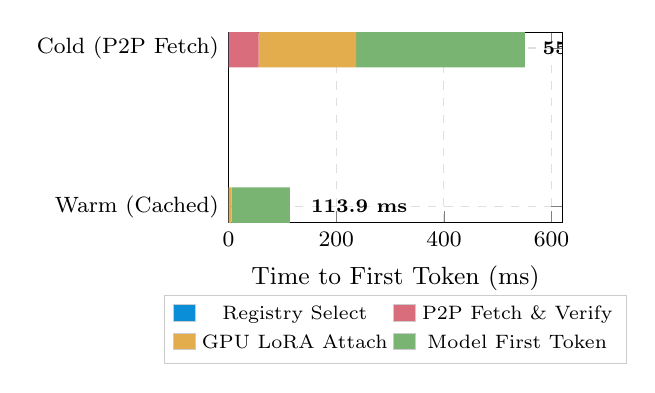
\begin{tikzpicture}
\begin{axis}[
    xbar stacked,
    width=0.48\textwidth,
    height=4.0cm,
    xmin=0, xmax=620,
    xlabel={Time to First Token (ms)},
    symbolic y coords={{Warm (Cached)}, {Cold (P2P Fetch)}},
    ytick=data,
    yticklabel style={font=\footnotesize},
    xticklabel style={font=\footnotesize},
    xlabel style={font=\small},
    bar width=14pt,
    legend style={font=\scriptsize, at={(0.5,-0.38)}, anchor=north, legend columns=2, draw=gray!40, fill=white},
    grid=major,
    grid style={dashed, gray!25}
]

% 1. Selection / Rank (<0.1ms)
\addplot[fill=cyan!75!blue, draw=none] coordinates {(0.05,{Warm (Cached)}) (0.03,{Cold (P2P Fetch)})};
% 2. P2P Download + Verify
\addplot[fill=vllmred!80, draw=none] coordinates {(0.08,{Warm (Cached)}) (55.92,{Cold (P2P Fetch)})};
% 3. LoRA Attach
\addplot[fill=boundorange!90, draw=none] coordinates {(5.54,{Warm (Cached)}) (180.80,{Cold (P2P Fetch)})};
% 4. Model Prefill (First Token)
\addplot[fill=traingreen!80, draw=none] coordinates {(108.23,{Warm (Cached)}) (313.61,{Cold (P2P Fetch)})};

\node at (axis cs:135,{Warm (Cached)}) [anchor=west, font=\scriptsize\bfseries] {113.9 ms};
\node at (axis cs:565,{Cold (P2P Fetch)}) [anchor=west, font=\scriptsize\bfseries] {550.4 ms};

\legend{Registry Select, P2P Fetch \& Verify, GPU LoRA Attach, Model First Token}
\end{axis}
\end{tikzpicture}

\caption{TTFT breakdown: cold P2P fetch vs. in-memory warm cache.}
\label{fig:latency_cold_warm}
\end{figure}

\section{Prompt Length Scaling}
\begin{figure*}[t]
\centering
% TikZ Figure: TTFT & MFU vs Prompt Length
% Usage: \input{tikzfigs/fig_latency_vs_prompt_length.tex}
% Self-contained color definitions
\providecolor{oursblue}{RGB}{46,111,183}
\providecolor{boundorange}{RGB}{224,164,58}
\providecolor{vllmred}{RGB}{209,73,91}
\providecolor{basegray}{RGB}{154,164,174}
\providecolor{traingreen}{RGB}{89,161,79}
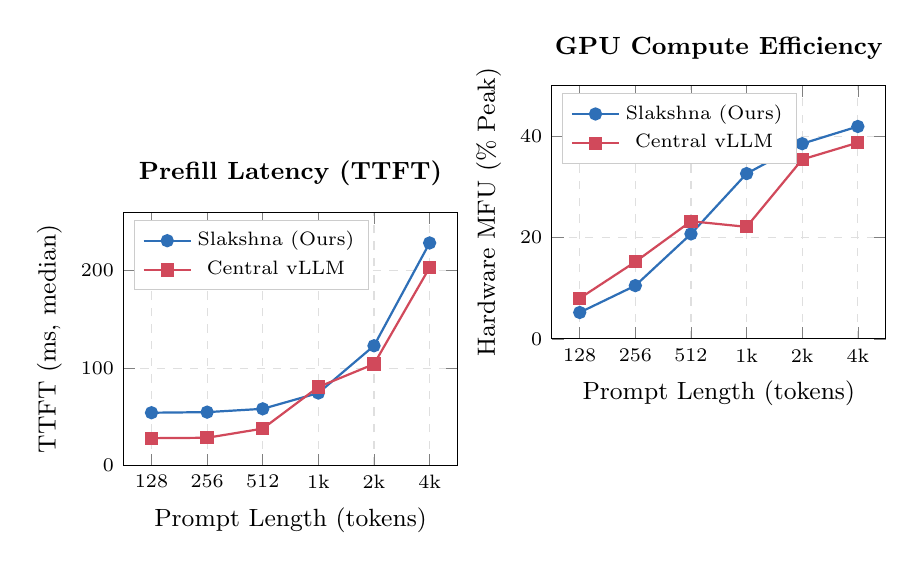
\begin{tikzpicture}
% Left Subplot: TTFT
\begin{axis}[
    name=ax1,
    width=0.48\textwidth,
    height=4.8cm,
    xmode=log,
    log basis x={2},
    xlabel={Prompt Length (tokens)},
    ylabel={TTFT (ms, median)},
    xtick={128, 256, 512, 1024, 2048, 4096},
    xticklabels={128, 256, 512, 1k, 2k, 4k},
    ymin=0, ymax=260,
    yticklabel style={font=\scriptsize},
    xticklabel style={font=\scriptsize},
    label style={font=\small},
    title style={font=\small\bfseries},
    title={Prefill Latency (TTFT)},
    grid=major,
    grid style={dashed, gray!25},
    legend style={font=\scriptsize, at={(0.03,0.97)}, anchor=north west, draw=gray!40, fill=white}
]
\addplot[color=oursblue, mark=*, thick] coordinates {
    (128, 54.2) (256, 54.8) (512, 58.2) (1024, 74.4) (2048, 122.9) (4096, 228.4)
};
\addplot[color=vllmred, mark=square*, thick] coordinates {
    (128, 28.1) (256, 28.5) (512, 37.9) (1024, 80.6) (2048, 104.1) (4096, 203.2)
};
\legend{Slakshna (Ours), Central vLLM}
\end{axis}

% Right Subplot: MFU (%)
\begin{axis}[
    name=ax2,
    at={($(ax1.east)+(1.2cm,0)$)},
    width=0.48\textwidth,
    height=4.8cm,
    xmode=log,
    log basis x={2},
    xlabel={Prompt Length (tokens)},
    ylabel={Hardware MFU (\% Peak)},
    xtick={128, 256, 512, 1024, 2048, 4096},
    xticklabels={128, 256, 512, 1k, 2k, 4k},
    ymin=0, ymax=50,
    yticklabel style={font=\scriptsize},
    xticklabel style={font=\scriptsize},
    label style={font=\small},
    title style={font=\small\bfseries},
    title={GPU Compute Efficiency},
    grid=major,
    grid style={dashed, gray!25},
    legend style={font=\scriptsize, at={(0.03,0.97)}, anchor=north west, draw=gray!40, fill=white}
]
\addplot[color=oursblue, mark=*, thick] coordinates {
    (128, 5.2) (256, 10.5) (512, 20.7) (1024, 32.6) (2048, 38.5) (4096, 41.9)
};
\addplot[color=vllmred, mark=square*, thick] coordinates {
    (128, 8.0) (256, 15.2) (512, 23.2) (1024, 22.1) (2048, 35.4) (4096, 38.7)
};
\legend{Slakshna (Ours), Central vLLM}
\end{axis}
\end{tikzpicture}

\caption{Prefill TTFT and hardware MFU as prompt length scales to 4k tokens.}
\label{fig:prompt_length}
\end{figure*}

\section{Decoding Speed and E2E Latency}
\begin{figure*}[t]
\centering
% TikZ Figure: TPOT & End-to-End Latency vs Output Length
% Usage: \input{tikzfigs/fig_latency_vs_output_length.tex}
% Self-contained color definitions
\providecolor{oursblue}{RGB}{46,111,183}
\providecolor{boundorange}{RGB}{224,164,58}
\providecolor{vllmred}{RGB}{209,73,91}
\providecolor{basegray}{RGB}{154,164,174}
\providecolor{traingreen}{RGB}{89,161,79}
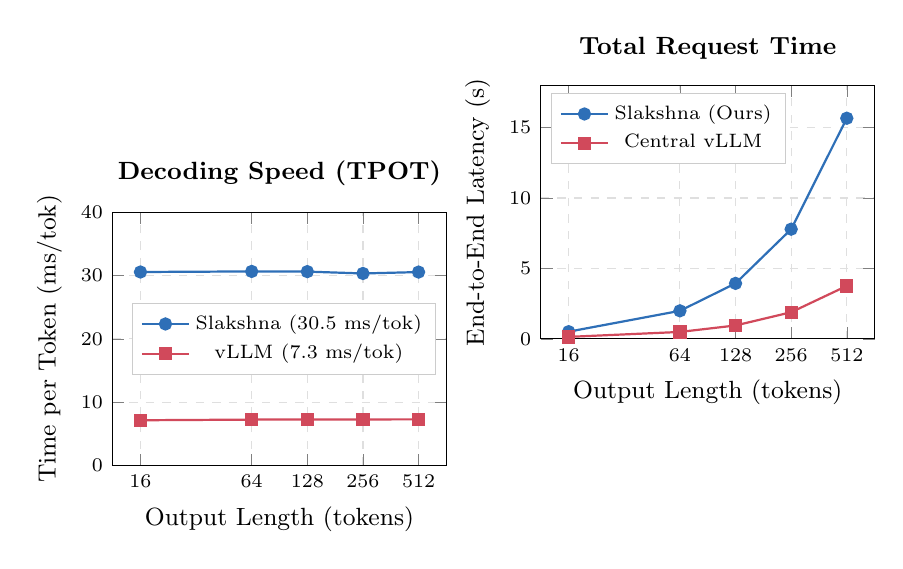
\begin{tikzpicture}
% Left Subplot: TPOT (ms/token)
\begin{axis}[
    name=ax1,
    width=0.48\textwidth,
    height=4.8cm,
    xmode=log,
    log basis x={2},
    xlabel={Output Length (tokens)},
    ylabel={Time per Token (ms/tok)},
    xtick={16, 64, 128, 256, 512},
    xticklabels={16, 64, 128, 256, 512},
    ymin=0, ymax=40,
    yticklabel style={font=\scriptsize},
    xticklabel style={font=\scriptsize},
    label style={font=\small},
    title style={font=\small\bfseries},
    title={Decoding Speed (TPOT)},
    grid=major,
    grid style={dashed, gray!25},
    legend style={font=\scriptsize, at={(0.97,0.50)}, anchor=east, draw=gray!40, fill=white}
]
\addplot[color=oursblue, mark=*, thick] coordinates {
    (16, 30.55) (64, 30.64) (128, 30.61) (256, 30.32) (512, 30.54)
};
\addplot[color=vllmred, mark=square*, thick] coordinates {
    (16, 7.15) (64, 7.25) (128, 7.27) (256, 7.28) (512, 7.29)
};
\legend{Slakshna (30.5 ms/tok), vLLM (7.3 ms/tok)}
\end{axis}

% Right Subplot: Total End-to-End Latency (s)
\begin{axis}[
    name=ax2,
    at={($(ax1.east)+(1.2cm,0)$)},
    width=0.48\textwidth,
    height=4.8cm,
    xmode=log,
    log basis x={2},
    xlabel={Output Length (tokens)},
    ylabel={End-to-End Latency (s)},
    xtick={16, 64, 128, 256, 512},
    xticklabels={16, 64, 128, 256, 512},
    ymin=0, ymax=18,
    yticklabel style={font=\scriptsize},
    xticklabel style={font=\scriptsize},
    label style={font=\small},
    title style={font=\small\bfseries},
    title={Total Request Time},
    grid=major,
    grid style={dashed, gray!25},
    legend style={font=\scriptsize, at={(0.03,0.97)}, anchor=north west, draw=gray!40, fill=white}
]
\addplot[color=oursblue, mark=*, thick] coordinates {
    (16, 0.51) (64, 1.99) (128, 3.94) (256, 7.79) (512, 15.67)
};
\addplot[color=vllmred, mark=square*, thick] coordinates {
    (16, 0.14) (64, 0.49) (128, 0.95) (256, 1.89) (512, 3.76)
};
\legend{Slakshna (Ours), Central vLLM}
\end{axis}
\end{tikzpicture}

\caption{Decoding TPOT and total latency across generated sequence lengths.}
\label{fig:output_length}
\end{figure*}

\section{Concurrency and Throughput}
\begin{figure*}[t]
\centering
% TikZ Figure: Throughput & Goodput vs Concurrency
% Usage: \input{tikzfigs/fig_throughput_vs_concurrency.tex}
% Self-contained color definitions
\providecolor{oursblue}{RGB}{46,111,183}
\providecolor{boundorange}{RGB}{224,164,58}
\providecolor{vllmred}{RGB}{209,73,91}
\providecolor{basegray}{RGB}{154,164,174}
\providecolor{traingreen}{RGB}{89,161,79}
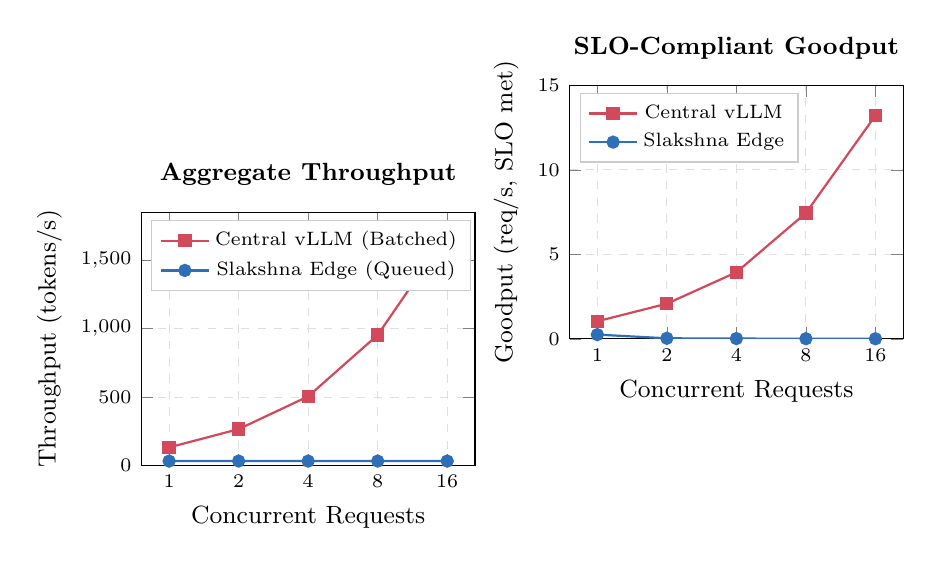
\begin{tikzpicture}
% Left: Throughput (tokens/s)
\begin{axis}[
    name=ax1,
    width=0.48\textwidth,
    height=4.8cm,
    xmode=log,
    log basis x={2},
    xlabel={Concurrent Requests},
    ylabel={Throughput (tokens/s)},
    xtick={1, 2, 4, 8, 16},
    xticklabels={1, 2, 4, 8, 16},
    ymin=0, ymax=1850,
    yticklabel style={font=\scriptsize},
    xticklabel style={font=\scriptsize},
    label style={font=\small},
    title style={font=\small\bfseries},
    title={Aggregate Throughput},
    grid=major,
    grid style={dashed, gray!25},
    legend style={font=\scriptsize, at={(0.03,0.97)}, anchor=north west, draw=gray!40, fill=white}
]
\addplot[color=vllmred, mark=square*, thick] coordinates {
    (1, 132.5) (2, 265.9) (4, 504.8) (8, 953.3) (16, 1692.0)
};
\addplot[color=oursblue, mark=*, thick] coordinates {
    (1, 32.5) (2, 32.8) (4, 32.5) (8, 32.6) (16, 32.6)
};
\legend{Central vLLM (Batched), Slakshna Edge (Queued)}
\end{axis}

% Right: Goodput (req/s meeting SLO)
\begin{axis}[
    name=ax2,
    at={($(ax1.east)+(1.2cm,0)$)},
    width=0.48\textwidth,
    height=4.8cm,
    xmode=log,
    log basis x={2},
    xlabel={Concurrent Requests},
    ylabel={Goodput (req/s, SLO met)},
    xtick={1, 2, 4, 8, 16},
    xticklabels={1, 2, 4, 8, 16},
    ymin=0, ymax=15,
    yticklabel style={font=\scriptsize},
    xticklabel style={font=\scriptsize},
    label style={font=\small},
    title style={font=\small\bfseries},
    title={SLO-Compliant Goodput},
    grid=major,
    grid style={dashed, gray!25},
    legend style={font=\scriptsize, at={(0.03,0.97)}, anchor=north west, draw=gray!40, fill=white}
]
\addplot[color=vllmred, mark=square*, thick] coordinates {
    (1, 1.04) (2, 2.08) (4, 3.94) (8, 7.45) (16, 13.22)
};
\addplot[color=oursblue, mark=*, thick] coordinates {
    (1, 0.25) (2, 0.032) (4, 0.016) (8, 0.008) (16, 0.004)
};
\legend{Central vLLM, Slakshna Edge}
\end{axis}
\end{tikzpicture}

\caption{Throughput and goodput scaling under concurrent request loads.}
\label{fig:concurrency}
\end{figure*}

\section{Fault Tolerance and Failover}
\begin{figure*}[t]
\centering
% TikZ Figure: Fault Tolerance Under Peer Crashes
% Usage: \input{tikzfigs/fig_fault_tolerance.tex}
% Self-contained color definitions
\providecolor{oursblue}{RGB}{46,111,183}
\providecolor{boundorange}{RGB}{224,164,58}
\providecolor{vllmred}{RGB}{209,73,91}
\providecolor{basegray}{RGB}{154,164,174}
\providecolor{traingreen}{RGB}{89,161,79}
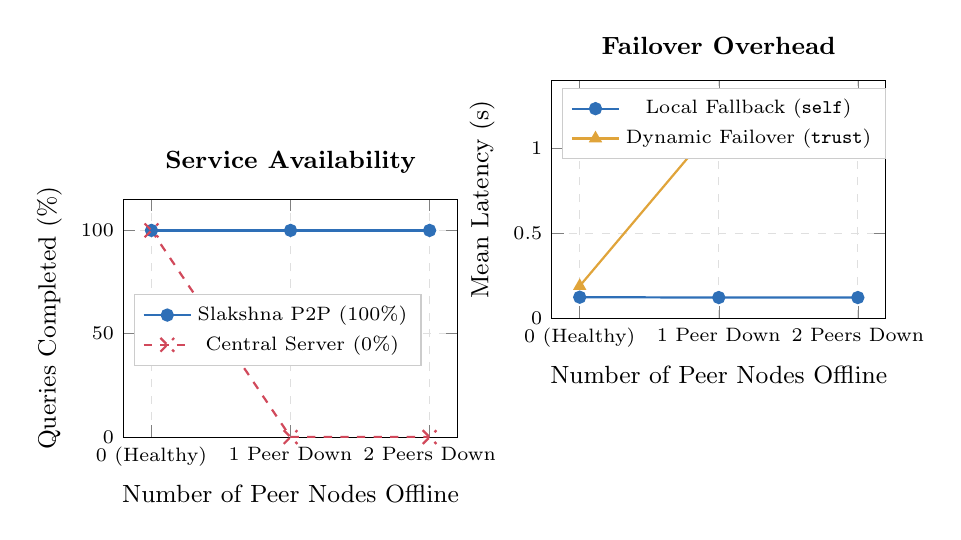
\begin{tikzpicture}
% Left: Availability (%)
\begin{axis}[
    name=ax1,
    width=0.48\textwidth,
    height=4.6cm,
    xlabel={Number of Peer Nodes Offline},
    ylabel={Queries Completed (\%)},
    xtick={0, 1, 2},
    xticklabels={0 (Healthy), 1 Peer Down, 2 Peers Down},
    ymin=0, ymax=115,
    yticklabel style={font=\scriptsize},
    xticklabel style={font=\scriptsize},
    label style={font=\small},
    title style={font=\small\bfseries},
    title={Service Availability},
    grid=major,
    grid style={dashed, gray!25},
    legend style={font=\scriptsize, at={(0.03,0.30)}, anchor=south west, draw=gray!40, fill=white}
]
\addplot[color=oursblue, mark=*, thick] coordinates {(0, 100) (1, 100) (2, 100)};
\addplot[color=vllmred, mark=x, thick, dashed, mark size=3.5pt] coordinates {(0, 100) (1, 0) (2, 0)};
\legend{Slakshna P2P (100\%), Central Server (0\%)}
\end{axis}

% Right: Latency (s)
\begin{axis}[
    name=ax2,
    at={($(ax1.east)+(1.2cm,0)$)},
    width=0.48\textwidth,
    height=4.6cm,
    xlabel={Number of Peer Nodes Offline},
    ylabel={Mean Latency (s)},
    xtick={0, 1, 2},
    xticklabels={0 (Healthy), 1 Peer Down, 2 Peers Down},
    ymin=0, ymax=1.4,
    yticklabel style={font=\scriptsize},
    xticklabel style={font=\scriptsize},
    label style={font=\small},
    title style={font=\small\bfseries},
    title={Failover Overhead},
    grid=major,
    grid style={dashed, gray!25},
    legend style={font=\scriptsize, at={(0.03,0.97)}, anchor=north west, draw=gray!40, fill=white}
]
\addplot[color=oursblue, mark=*, thick] coordinates {(0, 0.124) (1, 0.122) (2, 0.122)};
\addplot[color=boundorange, mark=triangle*, thick] coordinates {(0, 0.190) (1, 1.161) (2, 1.160)};
\legend{Local Fallback (\texttt{self}), Dynamic Failover (\texttt{trust})}
\end{axis}
\end{tikzpicture}

\caption{System availability and latency during peer node crashes.}
\label{fig:fault_tolerance}
\end{figure*}

\section{P2P Adapter Fetch vs Size}
\begin{figure}[h]
\centering
% TikZ Figure: Adapter Fetch & Attach vs File Size
% Usage: \input{tikzfigs/fig_fetch_vs_adapter_size.tex}
% Self-contained color definitions
\providecolor{oursblue}{RGB}{46,111,183}
\providecolor{boundorange}{RGB}{224,164,58}
\providecolor{vllmred}{RGB}{209,73,91}
\providecolor{basegray}{RGB}{154,164,174}
\providecolor{traingreen}{RGB}{89,161,79}
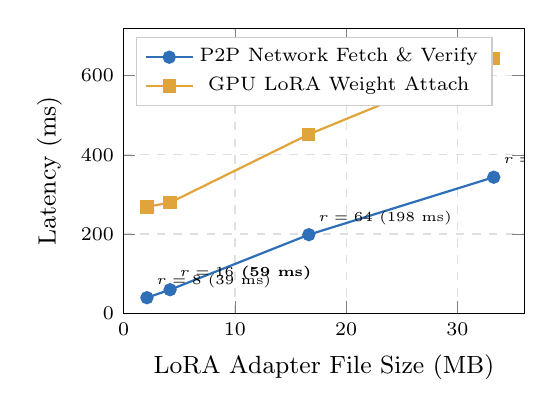
\begin{tikzpicture}
\begin{axis}[
    width=0.55\textwidth,
    height=5.2cm,
    xlabel={LoRA Adapter File Size (MB)},
    ylabel={Latency (ms)},
    ymin=0, ymax=720,
    xmin=0, xmax=36,
    xticklabel style={font=\scriptsize},
    yticklabel style={font=\scriptsize},
    label style={font=\small},
    grid=major,
    grid style={dashed, gray!25},
    legend style={font=\scriptsize, at={(0.03,0.97)}, anchor=north west, draw=gray!40, fill=white}
]
% Fetch + verify
\addplot[color=oursblue, mark=*, thick] coordinates {
    (2.09, 39.0) (4.17, 59.2) (16.64, 198.3) (33.26, 343.5)
};
% Attach
\addplot[color=boundorange, mark=square*, thick] coordinates {
    (2.09, 268.5) (4.17, 279.3) (16.64, 451.9) (33.26, 643.8)
};

\node at (axis cs:2.09,39.0) [anchor=south west, font=\tiny] {$r=8$ (39 ms)};
\node at (axis cs:4.17,59.2) [anchor=south west, font=\tiny\bfseries] {$r=16$ (59 ms)};
\node at (axis cs:16.64,198.3) [anchor=south west, font=\tiny] {$r=64$ (198 ms)};
\node at (axis cs:33.26,343.5) [anchor=south west, font=\tiny] {$r=128$ (344 ms)};

\legend{P2P Network Fetch \& Verify, GPU LoRA Weight Attach}
\end{axis}
\end{tikzpicture}

\caption{P2P transfer time vs. GPU attachment time across LoRA ranks.}
\label{fig:fetch_size}
\end{figure}

\section{Network Traffic and Privacy}
\begin{figure}[h]
\centering
% TikZ Figure: Network Traffic and Prompt Privacy
% Usage: \input{tikzfigs/fig_communication_bytes.tex}
% Self-contained color definitions
\providecolor{oursblue}{RGB}{46,111,183}
\providecolor{boundorange}{RGB}{224,164,58}
\providecolor{vllmred}{RGB}{209,73,91}
\providecolor{basegray}{RGB}{154,164,174}
\providecolor{traingreen}{RGB}{89,161,79}
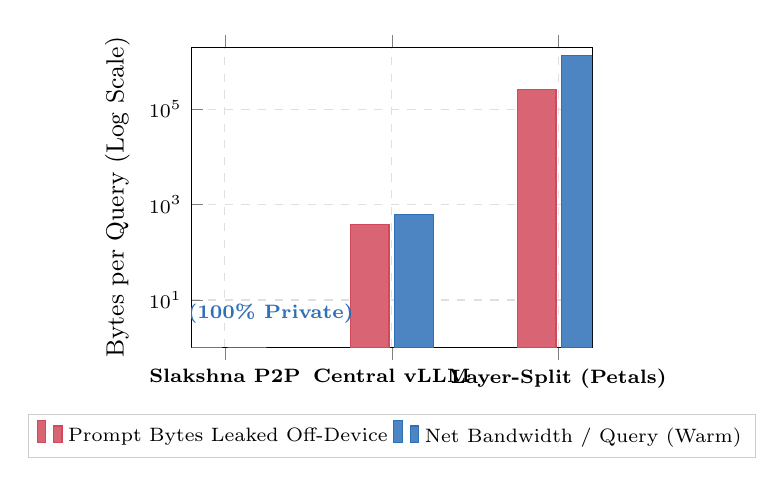
\begin{tikzpicture}
\begin{axis}[
    ybar,
    width=0.55\textwidth,
    height=5.4cm,
    ymode=log,
    log basis y={10},
    ymin=1, ymax=2000000,
    ylabel={Bytes per Query (Log Scale)},
    symbolic x coords={{Slakshna P2P}, {Central vLLM}, {Layer-Split (Petals)}},
    xtick=data,
    xticklabel style={font=\scriptsize\bfseries},
    yticklabel style={font=\scriptsize},
    label style={font=\small},
    bar width=14pt,
    legend style={font=\scriptsize, at={(0.5,-0.22)}, anchor=north, legend columns=2, draw=gray!40, fill=white},
    grid=major,
    grid style={dashed, gray!25}
]

% Prompt Bytes Sent Off-Device (0 for Slakshna -> plotted as 1 for log scale)
\addplot[fill=vllmred!85, draw=vllmred] coordinates {
    ({Slakshna P2P}, 1)
    ({Central vLLM}, 389)
    ({Layer-Split (Petals)}, 254540)
};

% Network Bytes per Warm Query (0 for Slakshna -> plotted as 1 for log scale)
\addplot[fill=oursblue!85, draw=oursblue] coordinates {
    ({Slakshna P2P}, 1)
    ({Central vLLM}, 608)
    ({Layer-Split (Petals)}, 1318779)
};

\node at (axis cs:{Slakshna P2P}, 2) [anchor=south, font=\scriptsize\bfseries, color=oursblue] {0 Bytes (100\% Private)};

\legend{Prompt Bytes Leaked Off-Device, Net Bandwidth / Query (Warm)}
\end{axis}
\end{tikzpicture}

\caption{Communication bytes per query and prompt data exposure.}
\label{fig:communication}
\end{figure}

\section{Dolly Generation Quality}
\begin{figure}[h]
\centering
% TikZ Figure: Dolly Open-Ended Generation Quality
% Usage: \input{tikzfigs/fig_dolly_generation_quality.tex}
% Self-contained color definitions
\providecolor{oursblue}{RGB}{46,111,183}
\providecolor{boundorange}{RGB}{224,164,58}
\providecolor{vllmred}{RGB}{209,73,91}
\providecolor{basegray}{RGB}{154,164,174}
\providecolor{traingreen}{RGB}{89,161,79}
\resizebox{\linewidth}{!}{%
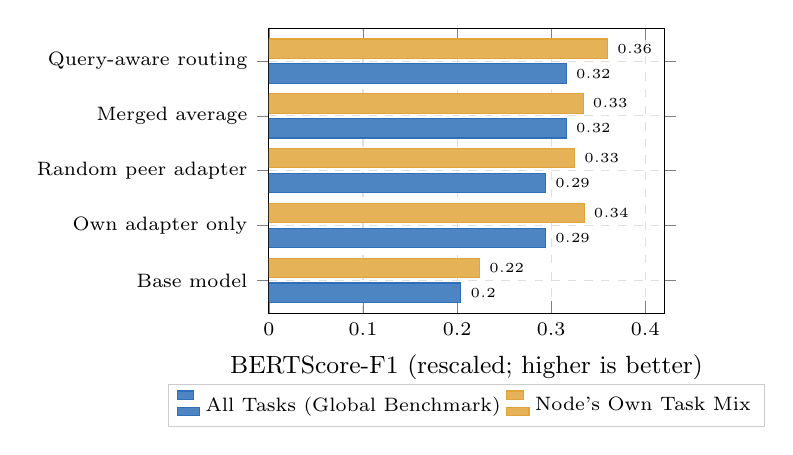
\begin{tikzpicture}
\begin{axis}[
    xbar,
    width=6.6cm,
    height=5.2cm,
    xmin=0, xmax=0.42,
    xlabel={BERTScore-F1 (rescaled; higher is better)},
    symbolic y coords={
        {Base model},
        {Own adapter only},
        {Random peer adapter},
        {Merged average},
        {Query-aware routing}
    },
    ytick=data,
    yticklabel style={font=\scriptsize, align=right},
    xticklabel style={font=\scriptsize},
    xlabel style={font=\small},
    nodes near coords,
    nodes near coords style={font=\tiny, text=black, anchor=west},
    nodes near coords align={horizontal},
    point meta=rawx,
    bar width=7pt,
    enlarge y limits=0.15,
    legend style={font=\scriptsize, at={(0.5,-0.25)}, anchor=north, legend columns=2, draw=gray!40, fill=white},
    grid=major,
    grid style={dashed, gray!25}
]

% All Tasks (Global Balanced Set)
\addplot[fill=oursblue!85, draw=oursblue] coordinates {
    (0.204,{Base model})
    (0.294,{Own adapter only})
    (0.294,{Random peer adapter})
    (0.316,{Merged average})
    (0.316,{Query-aware routing})
};

% Node's Own Mix (Local Task Skew)
\addplot[fill=boundorange!85, draw=boundorange] coordinates {
    (0.224,{Base model})
    (0.335,{Own adapter only})
    (0.325,{Random peer adapter})
    (0.334,{Merged average})
    (0.360,{Query-aware routing})
};

\legend{All Tasks (Global Benchmark), Node's Own Task Mix}
\end{axis}
\end{tikzpicture}%
}

\caption{Open-ended answer quality (BERTScore-F1) on Dolly-15k.}
\label{fig:dolly_quality}
\end{figure}

\end{document}
